\documentclass[11pt,a5paper,twoside,bahasa,listof=nochaptergap]{book}
\usepackage[tmargin=2.5cm,bmargin=2.5cm,lmargin=2.5cm,rmargin=2.0cm]{geometry}
\setcounter{secnumdepth}{5}
\usepackage[titletoc]{appendix}
\usepackage{csvsimple,longtable,booktabs}
\usepackage{listings}
\usepackage{diagbox}
\usepackage{csquotes}
\usepackage{tikz}
\usepackage{amsmath}
\usepackage[titles]{tocloft}

\begingroup
\makeatletter
\let\newcounter\@gobble\let\setcounter\@gobbletwo
\globaldefs\@ne \let\c@loldepth\@ne
\newlistof{listings}{lol}{\lstlistlistingname}
\newlistentry{lstlisting}{lol}{0}
\makeatother
\endgroup

\cftsetindents{lstlisting}{0in}{1.3in}

\lstset{ %
	numbers=left,
	xleftmargin=2mm,
	xrightmargin=2mm,
	frame=single,
	framesep=2mm,
	basicstyle=\footnotesize\ttfamily,
	framexleftmargin=2em,
	captionpos=b,
	belowcaptionskip=4pt,
	frame=single,
	breaklines=true,
	postbreak=\raisebox{0ex}[0ex][0ex]{\ensuremath{\color{red}\hookrightarrow\space}}
}
\usepackage{color, colortbl}
\definecolor{LightCyan}{rgb}{0.88,1,1}
\usepackage{rotating}
\usepackage{mdframed}
\usepackage{clrscode3e}
\usepackage[parfill]{parskip}
\usepackage{graphics}
\usepackage{fontspec}
\setsansfont{Trebuchet MS}
\setmainfont{Times New Roman}
\setmonofont{Courier New}
\usepackage{tocbibind}
\usepackage{enumitem}
\usepackage{pdflscape}
\usepackage{minted}
\usepackage{multirow}
\usepackage{graphicx}
\usepackage[verbose]{wrapfig}
\usepackage{changepage}
\usepackage{eso-pic}
\usepackage{ragged2e}
\usepackage{xesearch}
\usepackage[bahasa]{babel}
\usepackage[breaklinks=true]{hyperref}
\usepackage[font=small]{caption}
\usepackage{enumitem}
\setlist{nolistsep}
\usepackage{float}
\usepackage{longtable}
\usepackage{array,etoolbox}
\usepackage{amssymb}
\preto\tabular{\setcounter{magicrownumbers}{0}}
\preto\longtable{\setcounter{magicrownumbers}{0}}
\newcounter{magicrownumbers}
\newcommand\rownumber{\stepcounter{magicrownumbers}\arabic{magicrownumbers}}

\newcommand\nc[1]{%
	\multicolumn{1}{c}{#1}%
}

\newcommand\tab[1][1cm]{\hspace*{#1}}

\usepackage{setspace}
\singlespacing
\usepackage{fancyhdr}
\fancyhf{}
\renewcommand{\headrulewidth}{0pt}
\lhead[\thepage]{}
\rhead[]{\thepage}
\pagestyle{fancy}

\usepackage{titlesec}
\titleformat{\chapter}[display]{\filcenter\fontsize{11}{11}\bfseries}{\chaptername \ \thechapter}{0pt}{\filcenter\fontsize{11}{11}\bfseries\uppercase}
\titlespacing*{\chapter}{0pt}{-0.5cm}{40pt}
\titlespacing*{\section}{0pt}{11pt}{0pt}
\titlespacing*{\subsection}{0pt}{11pt}{0pt}
\titlespacing*{\subsubsection}{0pt}{11pt}{0pt}
\titleformat*{\section}{\fontsize{11}{11}\bfseries}
\titleformat*{\subsection}{\fontsize{11}{11}\bfseries}
\titleformat*{\subsubsection}{\fontsize{11}{11}\bfseries}


\addto\captionsbahasa{%
	\renewcommand\bibname{DAFTAR PUSTAKA}%
	\renewcommand\contentsname{DAFTAR ISI}%
	\renewcommand\listtablename{DAFTAR TABEL}%
	\renewcommand\listfigurename{DAFTAR GAMBAR}%
	\renewcommand\chaptername{BAB}%
}

\setlength{\parindent}{1cm}

\usepackage{chngcntr}
\renewcommand{\lstlistingname}{Kode Sumber}
\renewcommand{\lstlistlistingname}{DAFTAR KODE SUMBER}
\renewcommand*\thechapter{\arabic{chapter}}
\renewcommand\cftlstlistingpresnum{Kode Sumber }
\newcommand{\var}[2]{\newcommand{#1}{#2}}
\var{\judul}{Rancang Bangun Aplikasi "TPort" Sebagai Media Informasi Pencapaian Revenue Menggunakan Kerangka Kerja Laravel}
\var{\judulEnglish}{}

\var{\penulis}{Rohana Qudus }
\var{\nrp}{5115 100 045 }
\var{\penulisDua}{Rafi R. Ramadhan }
\var{\nrpDua}{5115 100 158 }
\var{\jurusan}{Informatika }
\var{\jurusanEnglish}{Informatics Department }
\var{\fakultas}{Teknologi Informasi dan Komunikasi }
\var{\fakultasEnglish}{Information Technology and Communication }
\var{\prodi}{S-1 }
\var{\pembimbingJurusan}{Ir. Muchammad Husni, M.Kom.}
\var{\nipPembimbingSatu}{19600221 198403 1 001}
\var{\pembimbingLapangan}{Herbintarto}
\var{\nipPembimbingDua}{195701011983031004}


\usepackage{caption}
\captionsetup[table]{labelsep=space}
\captionsetup[figure]{labelsep=space}
\captionsetup[lstlisting]{labelsep=space}

\setlength\cftparskip{-2pt}
\setlength\cftbeforechapskip{0pt}
\setlength{\lineskip}{0pt}

% Pemenggalan Tambahan
%english
%\hyphenation{ver-tex}
%\hyphenation{bridge}
%\hyphenation{block}
%\hyphenation{weight}
%\hyphenation{dis-joint}
%\hyphenation{par-ent}
%\hyphenation{root}
%\hyphenation{node}
%\hyphenation{set}
%\hyphenation{bridge-block}
%\hyphenation{con-nected}
%\hyphenation{com-po-nent}
%\hyphenation{undi-rected}
%\hyphenation{di-rected}
%\hyphenation{par-tially}
%\hyphenation{fully}
%\hyphenation{query}
%\hyphenation{dataset}

%bahasa
\hyphenation{me-nge-ta-hui}
\hyphenation{me-nya-ta-kan}
\hyphenation{meng-i-ni-si-al-i-sa-si}
\hyphenation{meng-gu-na-kan}
\hyphenation{me-la-ku-kan}
\hyphenation{me-li-bat-kan}
\hyphenation{permasalahan}

\makeatletter
\def\emptypage@emptypage{%
	\begin{center}
		\emph{Halaman ini sengaja dikosongkan}
	\end{center}
	\newpage%
}%
\def\cleardoublepage{%
	\clearpage%
	\if@twoside%
	\ifodd\c@page%
	% do nothing
	\else%
	\emptypage@emptypage%
	\fi%
	\fi%
}%
\makeatother
\raggedbottom


\renewcommand{\cftchapleader}{\cftdotfill{\cftdotsep}}
\renewcommand{\cftchappresnum}{BAB }
\renewcommand{\cfttabpresnum}{Tabel }
\cftsetindents{tab}{1em}{4.7em}
\renewcommand{\cftfigpresnum}{Gambar }
\cftsetindents{fig}{1em}{5.5em}

\cftsetindents{chapter}{0em}{3.6em}      % set amount of 
\cftsetindents{section}{2em}{2em}

\renewcommand{\thechapter}{\Roman{chapter}}
\renewcommand{\thesection}{\arabic{chapter}.\arabic{section}}
\renewcommand{\thesubsection}{\arabic{chapter}.\arabic{section}.\arabic{subsection}}
\renewcommand{\thefigure}{\arabic{chapter}.\arabic{figure}}
\renewcommand{\thetable}{\arabic{chapter}.\arabic{table}}

\newcommand{\insertfigure}{\begin{figure}\caption{A figure}\end{figure}}
\usepackage{etoolbox}% http://ctan.org/pkg/etoolbox
\makeatletter
% \patchcmd{<cmd>}{<search>}{<replace>}{<succes>}{<failure>}
\patchcmd{\@chapter}{\addtocontents{lof}{\protect\addvspace{10\p@}}}{}{}{}
\patchcmd{\@chapter}{\addtocontents{lot}{\protect\addvspace{10\p@}}}{}{}{}
\makeatother

\makeatletter
\g@addto@macro\appendix{%
	\addtocontents{toc}{%
		\protect\renewcommand{\protect\cftchappresnum}{}%
	}%
}
\makeatother


\renewcommand{\cftchapaftersnumb}{\hspace{0em}}

% Table caption above table
\floatstyle{plaintop}
\restylefloat{table}

% Centering table caption
\usepackage[justification=centering]{caption}
% Prevent hyphenation
\usepackage[none]{hyphenat}

\usepackage{mfirstuc}

\usepackage{tikz}

\begin{document} \sloppy
	% To prevent lstlisting from roman numbering
	\renewcommand{\thelstlisting}{\arabic{chapter}.\arabic{lstlisting}}
	\renewcommand{\theequation}{\arabic{chapter}.\arabic{equation}}
	
	% To remove spacing between chapter in list of figure and list of table
	\addtocontents{lof}{\protect\renewcommand*\protect\addvspace[1]{}}
	\addtocontents{lot}{\protect\renewcommand*\protect\addvspace[1]{}}
	
	% \setlength{\abovecaptionskip}{-12.75pt}
	
	\title {\judul}
	\author {\penulis}
	
	\frontmatter
	\addcontentsline{toc}{chapter}{SAMPUL}
	\newpage
	\newgeometry{top=7cm,left=2cm,bottom=2cm}

	\sffamily
	\thispagestyle{empty}
	\color{white}
	{ \noindent KERJA PRAKTIK - KI141330 }\\*[10pt] 
	{\large\textbf{\MakeUppercase{\judul}}} \\*[32pt]
	\\
	\\
	\MakeUppercase{\penulis} \\*
	NRP \nrp \\*[10pt]
	\MakeUppercase{\penulisDua} \\*
	NRP \nrpDua \\*[10pt]
	Dosen Pembimbing Jurusan \\*
	\pembimbingJurusan \\*[10pt]
	Pembimbing Lapangan \\*
	\pembimbingLapangan \\*[10pt]
	DEPARTEMEN \MakeUppercase{\jurusan} \\*
	Fakultas \fakultas \\*
	Institut Teknologi Sepuluh Nopember \\*
	Surabaya, 2018 \\*
	\AddToShipoutPictureBG*{
\includegraphics[width=\paperwidth,height=\paperheight]{sampul/sampul.png}}
	\rmfamily
	\normalsize
	\restoregeometry
	\color{black}
	\cleardoublepage
	
\newpage
	\newgeometry{top=7cm,left=2cm,bottom=2cm}

	\sffamily
	\thispagestyle{empty}
	{ \noindent KERJA PRAKTIK - KI141330 }\\*[10pt] 
	{\large\textbf{\MakeUppercase{\judul}}} \\*[32pt]
	\\
	\\
	\MakeUppercase{\penulis} \\*
	NRP \nrp \\*[10pt]
	\MakeUppercase{\penulisDua} \\*
	NRP \nrpDua \\*[10pt]
	Dosen Pembimbing Jurusan \\*
	\pembimbingJurusan \\*[10pt]
	Pembimbing Lapangan \\*
	\pembimbingLapangan \\*[10pt]
	DEPARTEMEN \MakeUppercase{\jurusan} \\*
	Fakultas \fakultas \\*
	Institut Teknologi Sepuluh Nopember \\*
	Surabaya, 2018 \\*
	\AddToShipoutPictureBG*{
\includegraphics[width=\paperwidth,height=\paperheight]{sampul/sampulWhite.png}}
	\rmfamily
	\normalsize
	\restoregeometry
	\color{black}
	\cleardoublepage

	\addcontentsline{toc}{chapter}{LEMBAR PENGESAHAN}
	\newpage
	\thispagestyle{plain}
	\begin{centering}
		\textbf{\MakeUppercase{\judul}} \\*[10pt]
		\textbf{\large{KERJA PRAKTIK}} \\*
		
		Oleh: \\*
		\textbf{\penulis} \\*
		NRP: \nrp \\*[20pt]
		\textbf{\penulisDua} \\*
		NRP: \nrpDua \\*[20pt]
	\end{centering}

	{\noindent Disetujui oleh Pembimbing Kerja Praktik:}\\*[20pt]         
	\pembimbingJurusan \hfill \hfill .......................... \\
		NIP: \nipPembimbingSatu \hfill \hfill (Pembimbing Jurusan) \\*[20pt]
		
	{\noindent \pembimbingLapangan  \hfill \hfill ...........................}  \\
	.\hfill \hfill (Pembimbing Lapangan) \\*[20pt] 

	\begin{centering}
		\textbf{SURABAYA} \\*
		\textbf{FEBRUARI 2018} \\*
	\end{centering}
	\cleardoublepage
	% INDONESIAN ABSTRAK
\addcontentsline{toc}{chapter}{ABSTRAK}
\thispagestyle{plain}
\begin{centering}
\textbf{\MakeUppercase{\judul}}
\end{centering}

\begin{tabular}{ll}
Nama  & : \MakeUppercase{\penulis} \\
NRP & : \nrp \\
Nama  & : \MakeUppercase{\penulisDua} \\
NRP & : \nrpDua \\
Departemen  & : Departemen \jurusan FTIK-ITS \\
Pembimbing Jurusan  & : Ir. Muchammad Husni, M.Kom. \\
Pembimbing Lapangan  & : \pembimbingLapangan
\end{tabular}
\\*[20pt]
\begin{centering}
\textbf{Abstrak}
\end{centering}
\itshape
% BEGIN
\\
\indent Telkomsel merupakan salah satu perusahaan operator telekomunikasi seluler di Indonesia.\\
\indent Pada laporan Kerja Praktik kali ini, penulis akan menguraikan secara garis besar pengerjaan aplikasi \textit{TPORT} yang menggunakan bahasa pemrograman HTML, CSS, JavaScript serta PHP.\\
\indent Berdasarkan hasil uji coba dan evaluasi menunjukkan bahwa aplikasi \textit{TPORT} yang dibuat telah berhasil memenuhi kebutuhan informasi yang dibutuhkan dalam memantau pencapaian revenue.
% END
\rm \\
\textbf{Kata Kunci: \textit{TPORT}, media informasi, pencapaian revenue}


\cleardoublepage

	\chapter{KATA PENGANTAR}

\indent\indent Puji syukur penulis panjatkan kepada Allah SWT. atas pimpinan, penyertaan, dan karunia-Nya sehingga penulis dapat menyelesaikan salah satu kewajiban penulis sebagai mahasiswa Teknik Informatika ITS yaitu Kerja Praktik yang berjudul :
\begin{center}
	\textbf{\MakeUppercase{\judul}}.
\end{center}

Penulis menyadari bahwa masih banyak kekurangan baik dalam pelaksanaan Kerja Praktik maupun penyusunan buku laporan ini. Namun penulis berharap buku laporan ini dapat menambah wawasan pembaca dan dapat menjadi sumber referensi.\\
Melalui buku laporan ini penulis juga ingin menyampaikan rasa terima kasih kepada orang-orang yang telah membantu dalam penyusunan laporan Kerja Praktik baik secara langsung maupun tidak langsung antara lain:
\begin{enumerate}
\item Kedua orang tua penulis.
\item Ibu Henning Titi C., S.Kom., M.Kom., selaku dosen pembimbing kerja praktik selama kerja praktik berlangsung.
\item Bapak Radityo Anggoro, S.Kom., M.Sc., Dr.Eng., selaku koordinator kerja praktik.
\item Bapak Nico Valiranzai selaku pembimbing lapangan selama kerja praktik berlangsung.
\end{enumerate}

\hfill Surabaya, Oktober 2017 \\ 

\begin{flushright}
\hfill{\penulis} 
\end{flushright}
\cleardoublepage

	\tableofcontents
	\cleardoublepage
	\listoftables
	\cleardoublepage
	\listoffigures
	\cleardoublepage
	\lstlistoflistings
	\cleardoublepage
	
	\mainmatter
	\chapter{PENDAHULUAN}

\section{Latar Belakang}
\tab PT Bank Rakyat Indonesia (BRI) merupakan satu-satunya Bank di dunia yang memilik satelit sendiri. Satelit yang dinamakan BRIsat ini diluncurkan dan mengorbit sejak 9 Juni 2016 lalu. Adanya satelit ini bertujuan untuk menjangkau nasabah BRI di seluruh Indonesia. Khususnya di daerah-daerah terpencil.
\tab Sebelumnya, untuk penanganan kebutuhan komunikasi data dengan ribuan kantor wilayah, kantor cabang, KCP, BRI Unit, Teras BRI dan 22.792 ATMnya, BRI menyewa transponder satelit lain. Dengan adanya satelit milik BRI sendiri, mulai diadakan relokasi ATM yang akan diarahkan kepada satelitnya sendiri.\\
\tab Kegiatan relokasi ini dalam sehari mencapai 100 titik atau lebih. Saat ini, untuk pencatatan kegiatan relokasinya hanya dilakukan dengan menggunakan \textit{tools} berupa Microsoft Excel. Oleh karena itu, dibutuhkan suatu sistem untuk memonitoring kegiatan relokasi ATM menuju BRIsat\cite{bri}.

\section{Tujuan}
Pembuatan Sistem Monitoring SIK ini bertujuan untuk:
\begin{enumerate}
\item Memudahkan monitoring kegiatan relokasi ATM
\item Melakukan efisiensi kerja 
\end{enumerate}

\section{Manfaat}
Manfaat dari pembuatan Sistem Monitoring SIK ini adalah sebagai berikut:

\begin{enumerate}
	\item Membuat pengerjaan monitoring relokasi ATM lebih efisien
	\item Membantu memudahkan kegiatan monitoring relokasi ATM
\end{enumerate}

\section{Rumusan Masalah}
Rumusan Masalah dari Kerja Praktik ini adalah sebagai berikut:

\begin{enumerate}
	\item Bagaimana menciptakan aplikasi web monitoring yang mudah dimengerti oleh pengguna?
	\item Bagaimana menciptakan aplikasi web monitoring yang dapat membantu efisiensi pengerjaan relokasi ATM?
\end{enumerate}

\section{Lokasi dan Waktu Kerja Praktik}
\tab Lokasi kerja praktik berada di PT. Bank Rakyat Indonesia dengan alamat Jalan RM. Harsono, RT 6/ RW 7, Ragunan, Pasar Minggu, Jakarta Selatan.\\
\tab Adapun kerja praktik dimulai pada tanggal 14 Juni 2017 hingga 9 Agustus 2017 dengan hari kerja Senin sampai Jumat pukul 07.30 sampai dengan pukul 16.30 WIB (8 jam kerja dan 1 jam istirahat).

\section{Metodologi}
Metodologi dalam pembuatan buku Kerja Praktik ini meliputi:
\begin{enumerate}
	\item \textbf{Perumusan Masalah}\\
	Untuk mengetahui domain dan fungsionalitas, dijelaskan secara rinci bagaimana sistem yang harus dibuat. Penjelasan oleh pembimbing kerja praktik kali ini menghasilkan beberapa catatan mengenai gambaran cara kerja sistem dan rincian kebutuhan sistem. Setelah mendapatkan gambaran sistem, diskusi lebih lanjut dilakukan guna menentukan DBMS, bahasa pemrograman, dan framework yang dipakai dalam pembuatan sistem.
	
	\item \textbf{Studi Literatur}\\
	Pada tahap ini, setelah ditentukannya DBMS, bahasa pemrograman sampai dengan framework yang digunakan, dilakukan studi literatur lanjut mengenai bagaimana penggunaannya dalam membangun sistem sesuai yang diharapkan.
	
	Secara garis besar, untuk membuat Monitoring SIK digunakan bahasa pemrograman HTML, CSS, Javascript dan PHP untuk back end sistem, serta DBMS MySQL sebagai penyimpanan data relokasi, yang dikemas	melalui framework Laravel.
	
	\item \textbf{Analisis dan Perancangan Sistem}\\
	Pada tahap ini akan dijelaskan tentang analisis serta perancangan sistem yang akan dibangun oleh penulis.
	
	\item \textbf{Implementasi Sistem}\\
	Implementasi merupakan tahap pembangunan rancangan. Pada tahap ini merealisasikan apa yang terjadi pada tahap sebelumnya, sehingga sesuai dengan apa yang telah direncanakan.
	
	\item \textbf{Pengujian dan Evaluasi}\\
	Pada tahap ini dilakukan uji coba pada aplikasi yang telah diimplementasikan. Tahap ini bermaksud untuk mengevaluasi kesesuaian sistem dan aplikasi yang dibuat apakah dapat dilakukan dengan lancar atau tidak. Selain itu juga untuk mencari masalah yang mungkin timbul dan tidak lupa mengadakan perbaikan jika terdapat kesalahan.
	
	\item \textbf{Kesimpulan dan Saran}\\
	Pengujian yang dilakukan ini telah memenuhi syarat yang diinginkan, dan berjalan dengan baik dan lancar.
\end{enumerate}

\section{Sistematika Laporan}
Laporan Kerja Praktik ini terbagi menjadi 7 bab dengan rincian sebagai berikut:
	\begin{enumerate}
	\item BAB I: PENDAHULUAN
	
	Bab ini berisi latar belakang, tujuan, manfaat, rumusan masalah, lokasi dan waktu kerja praktik, metodologi dan sistematika laporan.
		
	\item BAB II: PROFIL PERUSAHAAN
		
	Bab ini berisi gambaran umum PT Bank Rakyat Indonesia, mulai dari sejarah, tujuan, visi dan misi perusahaan, dan divisi tempat kerja praktik dilakukan.
		
	\item BAB III: TINJAUAN PUSTAKA
		
	Bab ini berisi dasar teori dari metode/teknologi yang digunakan dalam menyelesaikan proyek kerja praktik.
		
	\item BAB IV: ANALISIS DAN PERANCANGAN SISTEM
		
	Bab ini dijelaskan mengenai desain antarmuka aplikasi.
		
	\item BAB V: IMPLEMENTASI SISTEM
		
	Bab ini berisi uraian tahap-tahap yang dilakukan untuk proses implementasi aplikasi.
		
	\item BAB VI: HASIL DAN UJI COBA
	
	Bab ini berisi hasil uji coba dan evaluasi dari perangkat lunak yang telah dikembangkan selama pelaksanaan kerja praktik.
	
	\item KESIMPULAN DAN SARAN
	
	Bab ini berisi kesimpulan dan saran yang didapat dari proses pelaksanaan kerja praktik.
	\end{enumerate}

\cleardoublepage

	\chapter{PROFIL PERUSAHAAN}
\tab Sejak berdiri pada tanggal 26 Mei 1995, Telkomsel secara konsisten melayani negeri, menghadirkan akses telekomunikasi kepada masyarakat Indonesia yang tersebar dari Sabang sampai Merauke. \\
\tab Saat ini Telkomsel adalah operator selular terbesar di Indonesia dengan 178 juta pelanggan dan untuk melayani pelanggannya yang tersebar di seluruh Indonesia, termasuk juga di daerah terpencil dan pulau terluar serta daerah perbatasan negara, Telkomsel menggelar lebih dari 146 ribu BTS. \\
\tab Telkomsel secara konsisten mengimplementasikan teknologi seluler terkini dan menjadi yang pertama meluncurkan secara komersial layanan mobile 4G LTE di Indonesia. Memasuki era digital, Telkomsel terus mengembangkan bisnis digital, diantaranya Digital Advertising, Digital Lifestyle, Mobile Financial Services, dan Internet of Things. Untuk melayani kebutuhan pelanggan, Telkomsel menggelar call center 24 jam dan layanan GraPARI yang tersebar di seluruh Indonesia.\cite{telkomsel}.
\section{Visi, Misi dan Tujuan Perusahaan}
Visi, Misi dan Tujuan dari Telkomsel adalah sebagai berikut:
	\subsection{Visi Perusahaan}
	Menjadi penyedia layanan dan solusi gaya hidup digital mobile kelas dunia yang terpercaya.
	\subsection{Misi Perusahaan}
	Memberikan layanan dan solusi digital mobile yang melebihi ekspektasi para pengguna, menciptakan nilai lebih bagi para pemegang saham serta mendukung pertumbuhan ekonomi bangsa.\cite{aboutus}

\section{Sejarah Perusahaan}
\tab Pada tahun 1993 PT Telkom mulai merambah teknologi nirkabel GSM, di tahun selanjutnya, pada 1994 PT Satelit Palapa Indonesia operator jaringan GSM pertama di Indonesia yang mengeluarkan kartu SIM muncul. PT Telkomsel kemudian didirikan bersama Indosat pada tahun 1995 dan meluncurkan kartu Halo pada tanggal 26 Mei 1995 sebagai layanan paska bayar. Pada tahun 2015 Saham Telkomsel dimiliki oleh Telkom Indonesia sebesar 65\% dan sisanya oleh Singtel sebesar 35\%.\\
\tab Telkomsel menjadi operator telekomunikasi seluler terbesar di Indonesia dengan 139,3 juta pelanggan per 31 Desember 2014 dan pangsa pasar sebesar 51\% per 1 Januari 2007.[butuh rujukan] Jaringan Telkomsel telah mencakup 288 jaringan roaming internasional di 155 negara pada akhir tahun 2007. \\
\tab Saat ini Telkomsel menggelar lebih dari 100.000 BTS yang menjangkau sekitar 98\% wilayah populasi di Indonesia. Sebagai operator seluler nomor 6 terbesar di dunia dalam hal jumlah pelanggan, Telkomsel merupakan pemimpin pasar industri telekomunikasi di Indonesia yang kini dipercaya melayani lebih dari 143 juta pelanggan pada tahun 2015-2016. Dalam upaya memandu perkembangan industri telekomunikasi seluler di Indonesia memasuki era baru layanan mobile broadband, Telkomsel secara konsisten mengimplementasikan roadmap teknologi 3G, HSDPA, HSPA+, serta pengembangan jaringan Long Term Evolution (LTE). Kini Telkomsel mengembangkan jaringan broadband di 100 kota besar di Indonesia. Untuk membantu pelayanan kebutuhan pelanggan, Telkomsel kini didukung akses call center 24 jam dan 430 pusat layanan yang tersebar di seluruh Indonesia. Telkomsel bekerja pada jaringan 900/1.800 MHz.\cite{sejarahtsel}.

\section{Divisi Digital Regional Expansion Jawa Timur}
\tab Pada kesempatan kali ini, penulis ditempatkan pada Divisi Digital Regional Expansion Jawa Timur. Divisi ini berhubungan dengan layanan-layanan digital yang disediakan oleh Telkomsel. Di sini, penulis berkesempatan membuat Sistem Informasi untuk Memantau Pencapaian \textit{Revenue}.

\cleardoublepage
	\chapter{TINJAUAN PUSTAKA}

\section{Laravel}
\tab Laravel adalah sebuah framework PHP yang dirilis dibawah lisensi MIT, dibangun dengan konsep MVC (model view controller). Laravel adalah pengembangan website berbasis MVP yang ditulis dalam PHP yang dirancang untuk meningkatkan kualitas perangkat lunak dengan mengurangi biaya pengembangan awal dan biaya pemeliharaan, dan untuk meningkatkan pengalaman bekerja dengan aplikasi dengan menyediakan sintaks yang ekspresif, jelas dan menghemat waktu\cite{laravel}.\\
\tab Dalam pengerjaan aplikasi Monitoring SIK ini, digunakan \textit{framework} laravel untuk memudahkan pembuatan website. Laravel merupakan sebuah \textit{framework} yang dapat mencukupi kebutuhan pengguna. Karena membutuhkan waktu yang singkat dalam pengerjaan (\textit{development}), serta mudah untuk \textit{maintenance} sistem.

\section{Javascript}
\tab Javascript adalah sebuah bahasa pemrograman tingkat tinggi yang dinamis yang terkenal dengan first class functionnya yang artinya javascript memperlakukan sebuah function dengan porsi yang sama dengan variabel lainnya. Contohnya adalah pada bahasa pemrograman javascript, sebuah function dapat dijadikan parameter dari function yang lainnya. Javascript merupakan bahasa scripting untuk halaman web yang paling populer saat ini. Selain lingkungan browser, banyak pula platform lain yang menggunakan bahasa javascript seperti node.js dan apache CouchDB\cite{javascript}.\\
\tab Dalam pengerjaan aplikasi Monitoring SIK, dibutuhkan beberapa halaman dengan fitur untuk menampilkan beberapa pilihan yang hanya bisa dipilih apabila memilih fitur tertentu, oleh karena itu digunakan bahasa javascript untuk menampilkan pilihan tersebut.

\section{PHP}
\tab PHP adalah bahasa pemrograman yang mengelola web service yang menggunakan protokol HTTP. Web Service ini dibuat agar bisa dipanggil atau diakses oleh aplikasi lain melalui internet dengan menggunakan format pertukaran data sebagai format pengiriman pesan. File PHP ini berisi query untuk mengolah database yang akan di proses pada aplikasi\cite{PHP}.

\section{Apache HTTP Server}
\tab Dalam pembuatan Sistem Monitoring SIK ini, digunakan Apache HTTP Server sebagai server yang menjalankan sistem yang telah dibuat. Apache HTTP Server merupakan sebuah \textit{paltform web server}. Apache mendukung beberapa fitur, beberapa diimplementasikan sebagai modul yang dikompilasi. Perangkat ini berkisar dari bahasa pemrograman sisi server yang mendukung skema otentikasi. Beberapa antarmuka bahasa yang mendukung antara lain Perl, Python, Tcl dan PHP\cite{apache}.

\section{MySQL }
\tab Database pada sistem ini menggunakan MySQL. MySQL adalah sebuah perangkat lunak sistem manajemen basis data SQL. Database MySQL mendukung beberapa fitur seperti \textit{multithread}, \textit{multi-user}, dan SQL database manajemen sistem(DMBMS). Database ini digunakan untuk keperluan sistem database yang cepat, handal dan mudah digunakan\cite{mysql}.
	\chapter{ANALISIS DAN PERANCANGAN SISTEM}
\tab Pada bab ini akan dijelaskan mengenai desain dan implementasi rancangan sistem informasi untuk memantau pencapaian \textit{revenue} oleh Telkomsel Regional Jawa Timur. Sistem informasi untuk memantau pencapaian \textit{revenue} ini digunakan untuk memudahkan proses pengolahan data serta penyebaran informasi. Aplikasi web ini dikhususkan untuk internal Telkomsel.

\section{Mengelola Data \textit{Revenue}}
Berikut adalah deskripsi sistem dan diagram aktivitas pada \textit{use case} Mengelola Data \textit{Revenue}.

\subsection{Deskripsi Umum Sistem}
\tab Sistem akan menyimpan informasi mengenai data \textit{revenue}. Data yang dimasukkan akan disimpan ke dalam basis data. Pada kegiatan ini, terdapat sebuah parameter berupa cluster mana yang akan dimasukkan datanya ke basis data.

\subsection{\textit{Use Case} dan Fitur Sistem}
Gambar \ref{figure:use_case_mengelola_data_revenue} adalah \textit{use case} mengelola data \textit{revenue}. Pada pengelolaan data \textit{revenue}, pengguna dapat melakukan beberapa kegiatan sebagai berikut:

	\begin{figure}[h]
		\centerline {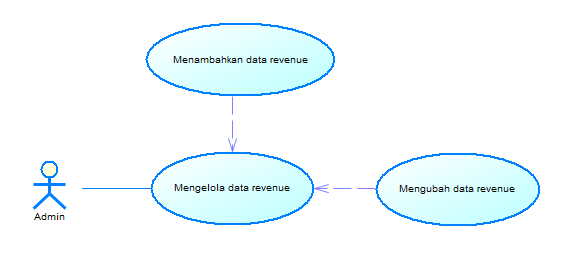
\includegraphics[width=8cm,height=4.5cm]{bab4/use_case_mengelola_data_revenue.png}}
		\caption{Diagram \textit{Use Case} Mengelola Data \textit{Revenue}}
		\label{figure:use_case_mengelola_data_revenue}
	\end{figure}
	
\subsubsection{Menambah Data \textit{Revenue}}
Pengguna dapat menambahkan data \textit{revenue}. Diagram \ref{figure:activity_menambah_data_revenue} adalah diagram aktivitas menambah data \textit{revenue} pada sistem TPORT. Pada pengisian form untuk mengupload data \textit{revenue}, pengguna harus menentukan rentang waktu data yang tersedia serta \textit{cluster} mana yang akan diupload datanya.
	
	\begin{figure}[h]
	\centerline {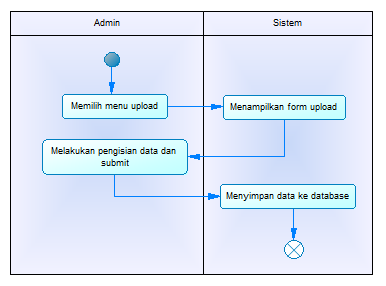
\includegraphics[width=8cm,height=6cm]{bab4/activity_menambah_data_revenue.png}}
	\caption{Diagram Aktivitas Menambah Data \textit{Revenue}}
	\label{figure:activity_menambah_data_revenue}
	\end{figure}
		
\subsubsection{Mengubah Data \textit{Revenue}}
Pengguna dapat mengubah data \textit{revenue}. Diagram \ref{figure:activity_mengubah_data_revenue} adalah diagram aktivitas mengubah data \textit{revenue} pada sistem TPORT. Untuk mengubah data yang sudah diupload, pengguna harus melakukan \textit{step} yang sama seperti menambahkan data baru. Sistem akan secara otomatis menggantikan data lama dengan data yang baru.
	
	\begin{figure}[h]
	\centerline {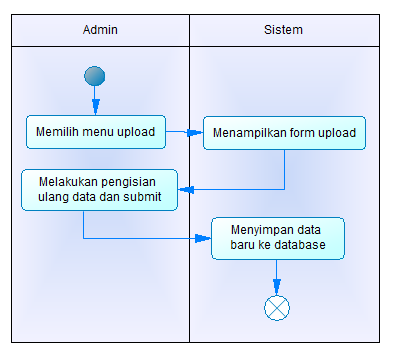
\includegraphics[width=7cm,height=6cm]{bab4/activity_mengubah_data_revenue.png}}
	\caption{Diagram Aktivitas Mengubah Data \textit{Revenue}}
	\label{figure:activity_mengubah_data_revenue}
	\end{figure}

\subsubsection{Menghapus Data \textit{Revenue}}
Sistem dapat menghapus data \textit{revenue}. Diagram \ref{figure:activity_menghapus_data_revenue} adalah diagram aktivitas menghapus data \textit{revenue} pada sistem TPORT. Sistem akan secara otomatis menghapus data \textit{revenue} dengan rentang waktu 23 bulan sejak tanggal sistem saat ini. 
	
	\begin{figure}[h]
		\centerline {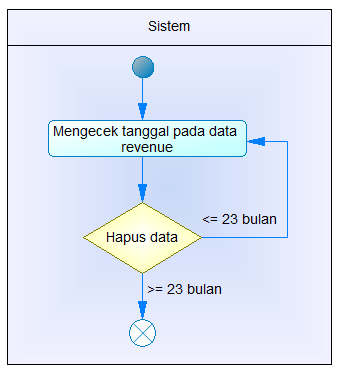
\includegraphics[width=5cm,height=6cm]{bab4/activity_menghapus_data_revenue.png}}
		\caption{Diagram Aktivitas Mengubah Data \textit{Revenue}}
		\label{figure:activity_menghapus_data_revenue}
	\end{figure}
	
\section{Mengelola Target Pencapaian \textit{Revenue}}
Berikut adalah deskripsi dan diagram aktivitas pada \textit{use case} Mengelola Target Pencapaian \textit{Revenue}.

\subsection{Deskripsi Umum Sistem}
\tab Sistem ini akan melakukan pengelolaan target pencapaian \textit{revenue}. Pada kegiatan ini, terdapat sebuah parameter berupa cluster mana yang akan ditentukan targetnya. Data yang dimasukkan akan disimpan ke dalam basis data.

\subsection{\textit{Use Case} dan Fitur Sistem}
Gambar \ref{figure:use_case_mengelola_target_pencapaian} adalah \textit{use case} mengelola target pencapaian \textit{revenue}. Pada pengelolaan target pencapaian \textit{revenue}, pengguna dapat melakukan beberapa kegiatan sebagai berikut:

	\begin{figure}[h]
		\centerline {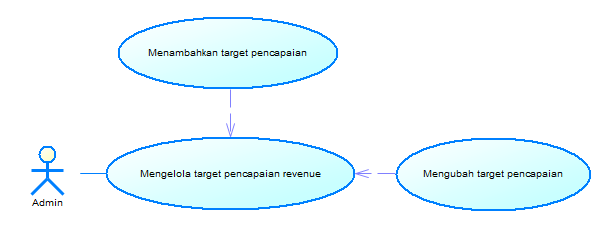
\includegraphics[width=10cm,height=4cm]{bab4/use_case_mengelola_target_pencapaian_revenue.png}}
		\caption{Diagram \textit{Use Case} Mengelola Target Pencapaian \textit{Revenue}}
		\label{figure:use_case_mengelola_target_pencapaian}
	\end{figure}

\subsubsection{Menambah Target Pencapaian \textit{Revenue}}
Pengguna dapat menambahkan target pencapaian \textit{revenue} untuk tiap cluster yang ada. Diagram \ref{figure:activity_menambah_target_pencapaian_revenue} adalah diagram aktivitas menambah target pencapaian \textit{revenue} pada sistem TPORT.
	
	\begin{figure}[h]
	\centerline {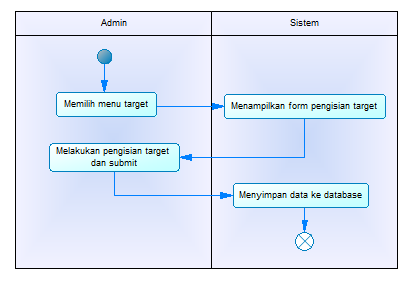
\includegraphics[width=9cm,height=6cm]{bab4/activity_menambah_target_pencapaian_revenue.png}}
	\caption{Diagram Aktivitas Menambah Target Pencapaian \textit{Revenue}}
	\label{figure:activity_menambah_target_pencapaian_revenue}
	\end{figure}
		
\subsubsection{Mengubah Target Pencapaian \textit{Revenue}}
User dapat mengubah data target pencapaian yang telah ditambahkan. Diagram \ref{figure:activity_mengubah_target_pencapaian_revenue} adalah diagram aktivitas mengubah target pencapaian \textit{revenue} pada sistem TPORT.
	
	\begin{figure}[h]
	\centerline {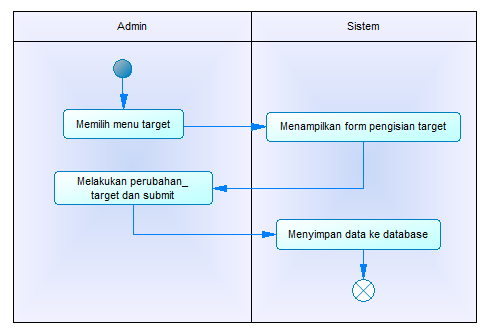
\includegraphics[width=9cm,height=5.6cm]{bab4/activity_mengubah_target_pencapaian_revenue.png}}
	\caption{Diagram Aktivitas Mengubah Target Pencapaian \textit{Revenue}}
	\label{figure:activity_mengubah_target_pencapaian_revenue}
	\end{figure}
		
\section{Melihat Hasil Pencapaian \textit{Revenue}}
Berikut adalah deskripsi dan diagram aktivitas pada \textit{use case} Melihat Hasil Pencapaian \textit{Revenue}.

\subsection{Deskripsi Umum Sistem}
\tab Sistem dapat menampilkan hasil pencapaian \textit{revenue} sesuai dengan kategori yang dipilih oleh pengguna.

\subsection{\textit{Use Case} dan Fitur Sistem}
Gambar \ref{figure:use_case_melihat_hasil_pencapaian_revenue} adalah \textit{use case} melihat hasil pencapaian \textit{revenue}. Pada halaman \textit{request}, pengguna dapat memilih kategori mana yang ingin dilihat hasilnya. Pengguna dapat melakukan beberapa kegiatan sebagai berikut:

	\begin{figure}[h!]
		\centerline
		{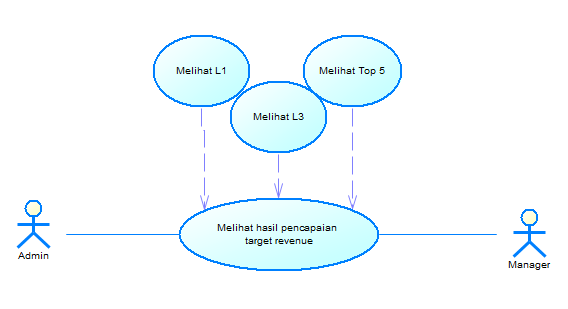
\includegraphics[width=9cm,height=5cm]{bab4/use_case_melihat_target_pencapaian_revenue.png}}
		\caption{Diagram \textit{Use Case} Melihat Target Pencapaian \textit{Revenue}}
		\label{figure:use_case_melihat_hasil_pencapaian_revenue}
	\end{figure}
	
\subsubsection{Melihat L1}
Pengguna dapat melihat target pencapaian \textit{revenue} berdasarkan L1. Diagram \ref{figure:activity_melihat_finish} adalah diagram aktivitas melihat target pencapaian \textit{revenue} sesuai kategori L1.

	\begin{figure}[h]
	\centerline {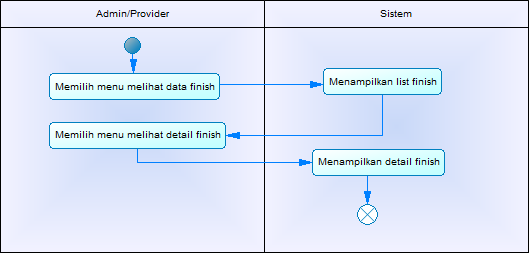
\includegraphics[width=9cm,height=5.5cm]{bab4/ActivityDiagram_MelihatFinish.png}}
	\caption{Diagram Aktivitas Melihat Daftar Permintaan Relokasi Sudah Dibayar}
	\label{figure:activity_melihat_finish}
	\end{figure}

\subsubsection{Melihat L3}
Pengguna dapat melihat target pencapaian \textit{revenue} berdasarkan L3. Diagram \ref{figure:activity_melihat_finish} adalah diagram aktivitas melihat target pencapaian \textit{revenue} sesuai kategori L3.

\begin{figure}[h]
	\centerline {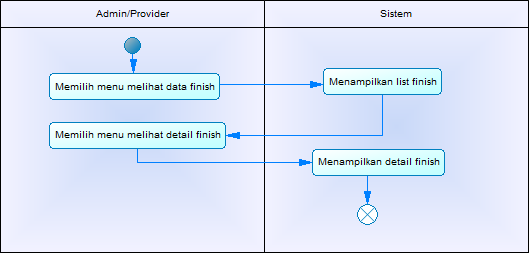
\includegraphics[width=9cm,height=5.5cm]{bab4/ActivityDiagram_MelihatFinish.png}}
	\caption{Diagram Aktivitas Melihat Daftar Permintaan Relokasi Sudah Dibayar}
	\label{figure:activity_melihat_finish}
\end{figure}

\subsubsection{Melihat Top 5}
Pengguna dapat melihat 5 pencapaian \textit{revenue} tertinggi berdasarkan perhitungan pada kategori L3. Diagram \ref{figure:activity_melihat_finish} adalah diagram aktivitas melihat 5 pencapaian \textit{revenue} tertinggi.

\begin{figure}[h]
	\centerline {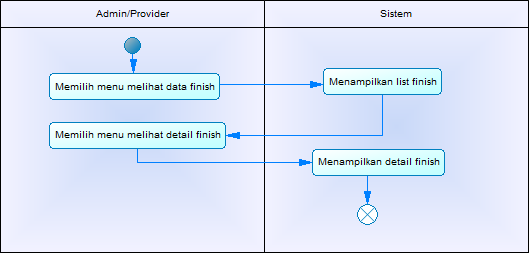
\includegraphics[width=9cm,height=5.5cm]{bab4/ActivityDiagram_MelihatFinish.png}}
	\caption{Diagram Aktivitas Melihat Daftar Permintaan Relokasi Sudah Dibayar}
	\label{figure:activity_melihat_finish}
\end{figure}
	
\newpage
\section{Perancangan Data}
\tab Dalam pembuatan sebuah sistem informasi, database merupakan salah satu faktor utama yang penting. Perancangan dan alur data pada sebuah sistem harus dapat memenuhi kebutuhan-kebutuhan sistem, meliputi penambahan data, perubahan isi data dan penghapusan data dari basis data sistem. Berikut adalah perancangan data pada sistem informasi TPORT.

\subsection{\textit{Conceptual Data Model}}
CDM (\textit{Conceptual Data Model}) merupakan sebuah model yang didasarkan pada objek-objek di dunia nyata. Objek dasar tersebut direpresentasikan dalam bentuk \textit{entity relationship diagram}. Gambar \ref{figure:CDM} adalah CDM pada pembuatan Aplikasi TPORT.

	\begin{figure}[h!]
	\centerline
	{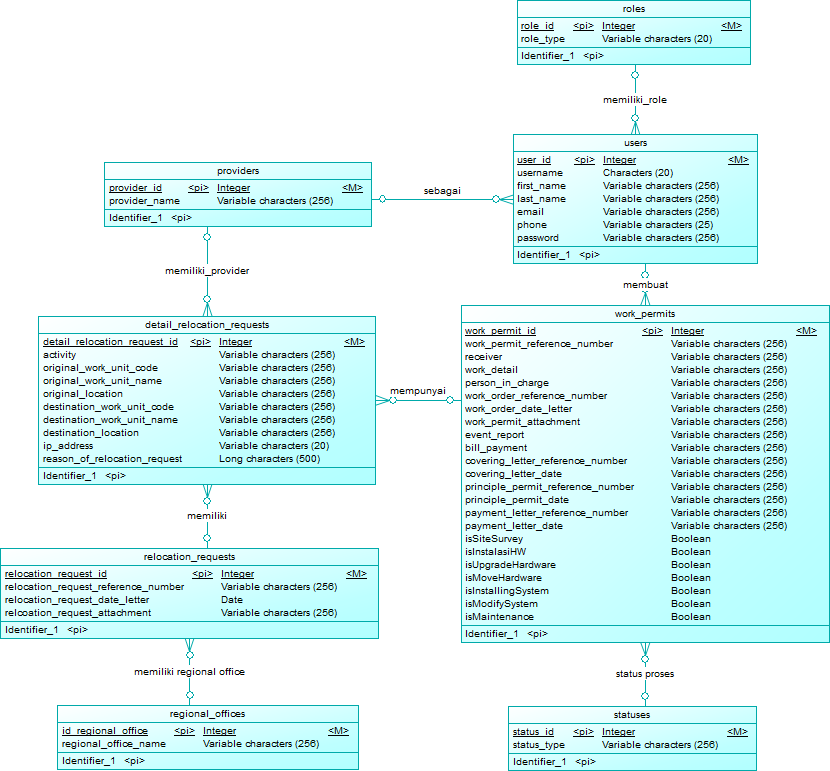
\includegraphics[width=10cm,height=14cm]{bab4/CDM.png}}
	\caption{Diagram \textit{Conceptual Data Model}}
	\label{figure:CDM}
	\end{figure}
	

	\chapter{IMPLEMENTASI}
Pada bab ini akan dipaparkan implementasi dari sistem yang dibangun. Bahasa pemrograman yang digunakan adalah HTML, CSS, Javascript, dan PHP yang dikemas dalam framework Laravel.

\section{Lingkungan Implementasi}
\tab Lingkungan implementasi dalam pembuatan sistem pada kerja praktik kali ini meliputi perangkat keras dan perangkat lunak yang digunakan untuk mengimplementasikan sistem yang telah dirancang adalah sebagai berikut:
\begin{enumerate}
	\item Perangkat Keras
	\begin{itemize}
	\item \textit{Processor} Intel® Core™ i7-5500U CPU @ 2.40GHz
	\item Memori 4 GB
	\end{itemize}
	\item Perangkat Lunak
	\begin{itemize}
	\item Sistem Operasi Ubuntu 16.04 LTS 64 bit.
	\item \textit{Text editor} Visual Studio Code
	\item Bahasa pemrograman PHP.
	\end{itemize}
\end{enumerate}

\section{Tampilan Fitur Aplikasi TPORT}
Berikut adalah tampilan aplikasi TPORT.

\subsection{Tampilan Halaman \textit{Request} TPORT}
Tampilan halaman \textit{request} TPORT menggunakan bahasa pemrograman HTML, CSS, Javascript dan PHP untuk tampilan sistem. Penampilan data pada halaman ini bersifat dinamis. Semua fitur pada aplikasi TPORT didaftar secara rinci dan dikemas dalam tampilan statis. Kemudian ketika salah satu fitur dipilih oleh user, maka akan diarahkan pada halaman sesuai fitur yang dipilih. Gambar \ref{figure:requestTPORT} dan \ref{figure:detailRequestTPORT} adalah tampilan halaman dan \ref{lst:request} adalah potongan kode dari halaman \textit{request} TPORT.

\begin{figure}[h!]
	\centerline
	{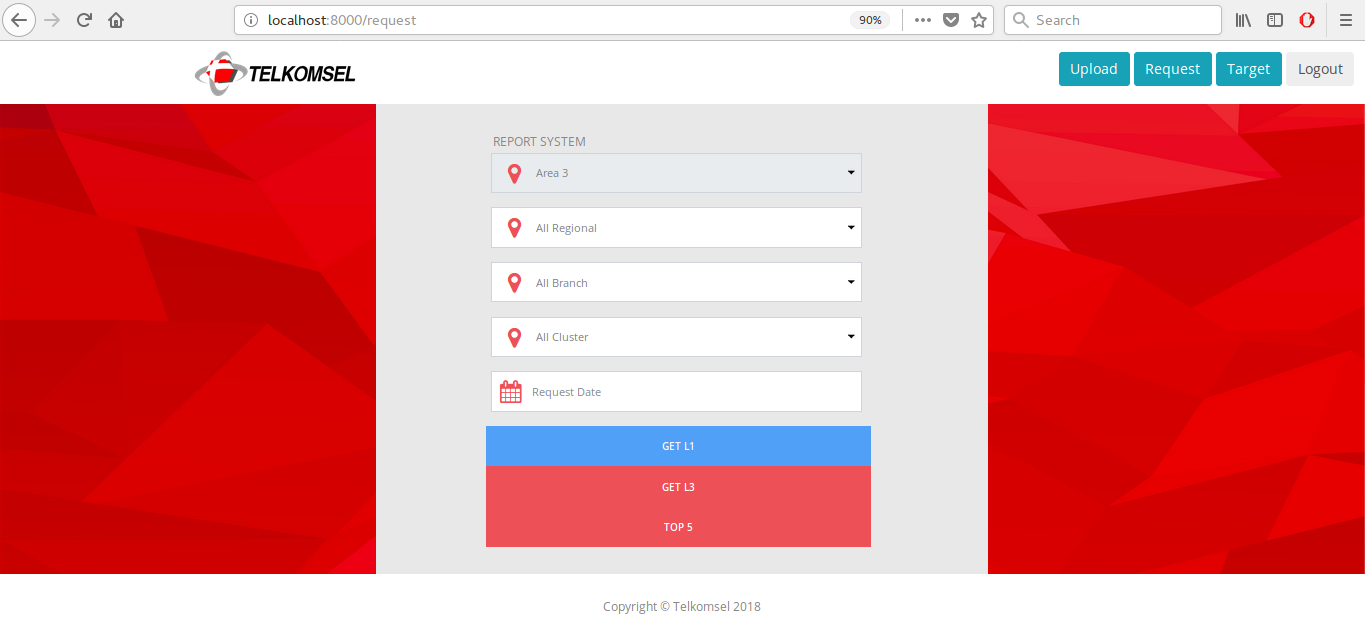
\includegraphics[width=10cm,height=5cm]{bab5/tampilanRequest.png}}
	\caption{Halaman \textit{Request} TPORT}
	\label{figure:requestTPORT}
\end{figure}

\begin{figure}[h!]
	\centerline
	{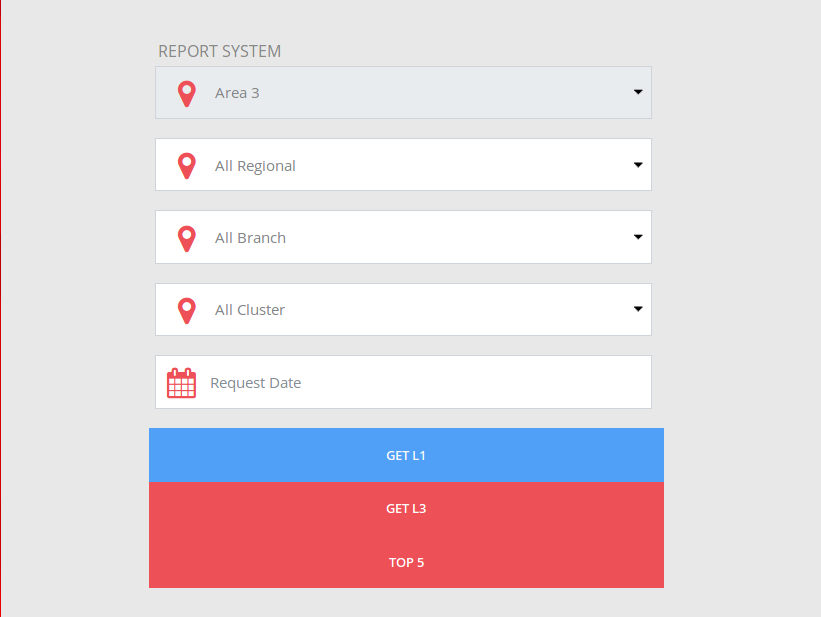
\includegraphics[width=10.5cm,height=7.5cm]{bab5/detailTampilanRequest.png}}
	\caption{Detail \textit{Form} pada Halaman \textit{Request} TPORT}
	\label{figure:detailRequestTPORT}
\end{figure}

\lstinputlisting[language=PHP, firstline=1, lastline=21, firstnumber=1, caption=Potongan Kode Tampilan Halaman \textit{Request} TPORT, label={lst:request}]{bab5/src/halamanReport.php}

\subsection{Tampilan Halaman \textit{Upload} TPORT}
Pada halaman menambahkan \textit{upload} TPORT bahasa yang digunakan adalah HTML, CSS, PHP dan Javascript. Sebuah \textit{form} akan ditampilkan dan kemudian pengguna akan mengisikan data-data sesuai spesifikasi file yang diupload. File yang diupload berupa file .csv (\textit{Comma Separated Values}). \textit{Form} tersebut akan menampung data-data yang diperlukan, kemudian akan disimpan ke dalam basis data sistem. Gambar \ref{figure:uploadTPORT} dan \ref{figure:detailUploadTPORT} adalah tampilan halaman \textit{upload} dan \ref{lst:uploadTPORT} adalah potongan kode halaman \textit{upload} TPORT.

\begin{figure}[h!]
\centerline
{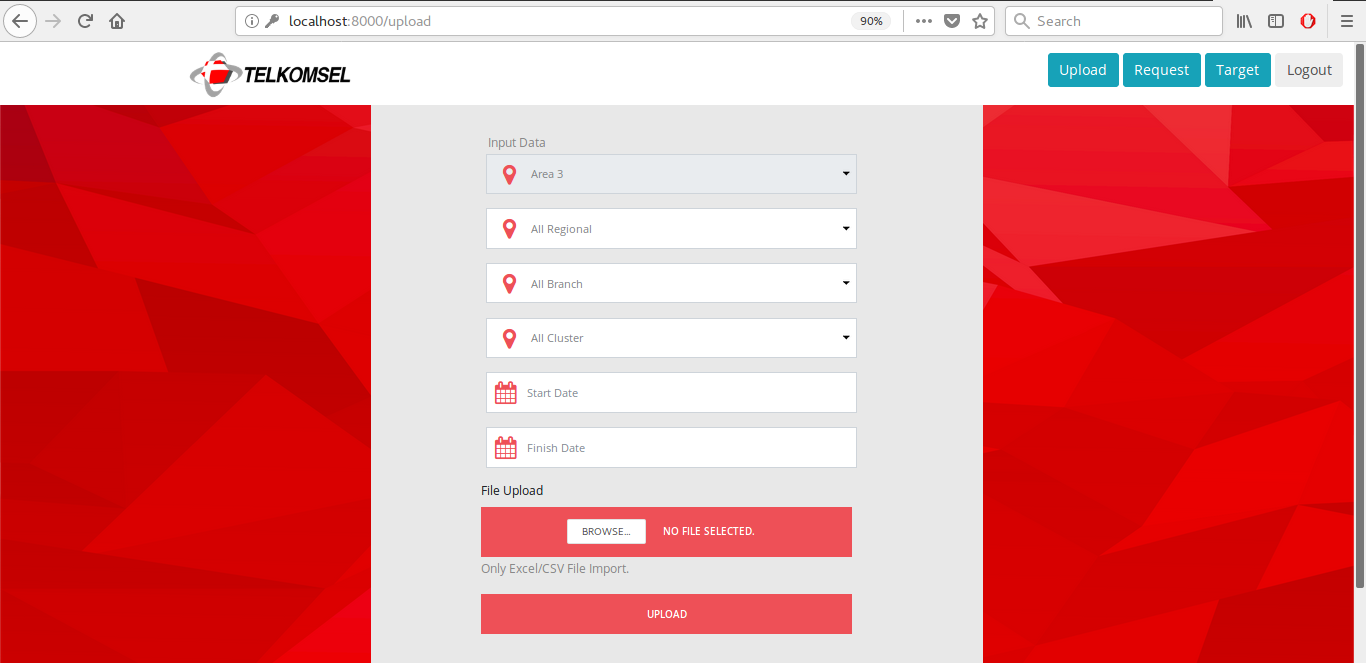
\includegraphics[width=10cm,height=5cm]{bab5/tampilanUpload.png}}
\caption{Halaman \textit{Upload} TPORT}
\label{figure:uploadTPORT}
\end{figure}

\begin{figure}[h!]
	\centerline
	{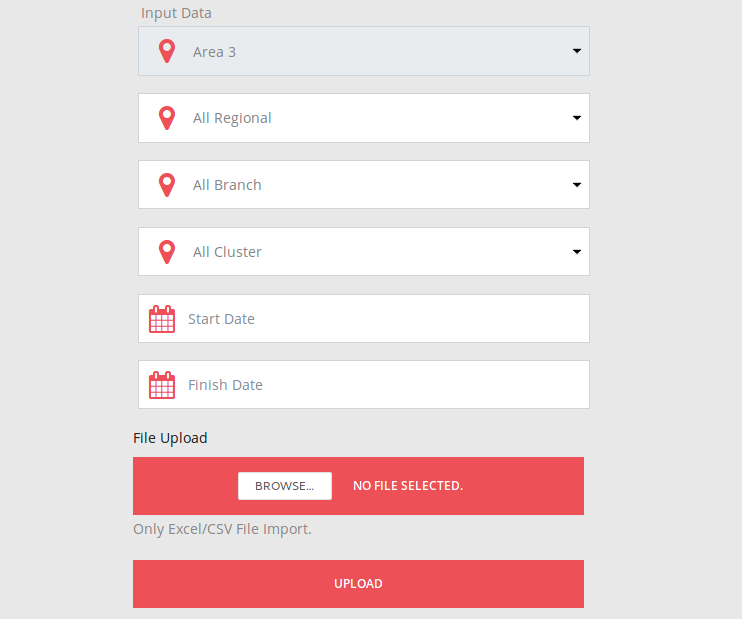
\includegraphics[width=10.5cm,height=7.5cm]{bab5/detailTampilanUpload.png}}
	\caption{Detail \textit{Form} pada Halaman \textit{Upload} TPORT}
	\label{figure:detailUploadTPORT}
\end{figure}


\lstinputlisting[language=PHP, firstline=1, lastline=59, firstnumber=1, caption=Potongan Kode Tampilan \textit{Upload} TPORT, label={lst:uploadTPORT}]{bab5/src/halamanUpload.php}

\subsection{Tampilan Halaman Target TPORT}
Pada halaman target TPORT bahasa yang digunakan adalah HTML, CSS, PHP dan Javascript. Sebuah \textit{form} akan ditampilkan kemudian pengguna mengisikan nilai \textit{revenue} sesuai target yang ingin diraih untuk tiap kluster. \textit{Form} tersebut akan menampung data-data yang diperlukan, kemudian akan disimpan ke dalam basis data sistem. Gambar \ref{figure:targetTPORT} dan \ref{figure:detailTargetTPORT} adalah tampilan halaman dan \ref{lst:targetTPORT} adalah potongan kode dari halaman target.

\lstinputlisting[language=PHP, firstline=1, lastline=43, firstnumber=1, caption=Potongan Kode Tampilan Target TPORT, label={lst:targetTPORT}]{bab5/src/halamanTarget.php}

\begin{figure}[h!]
	\centerline
	{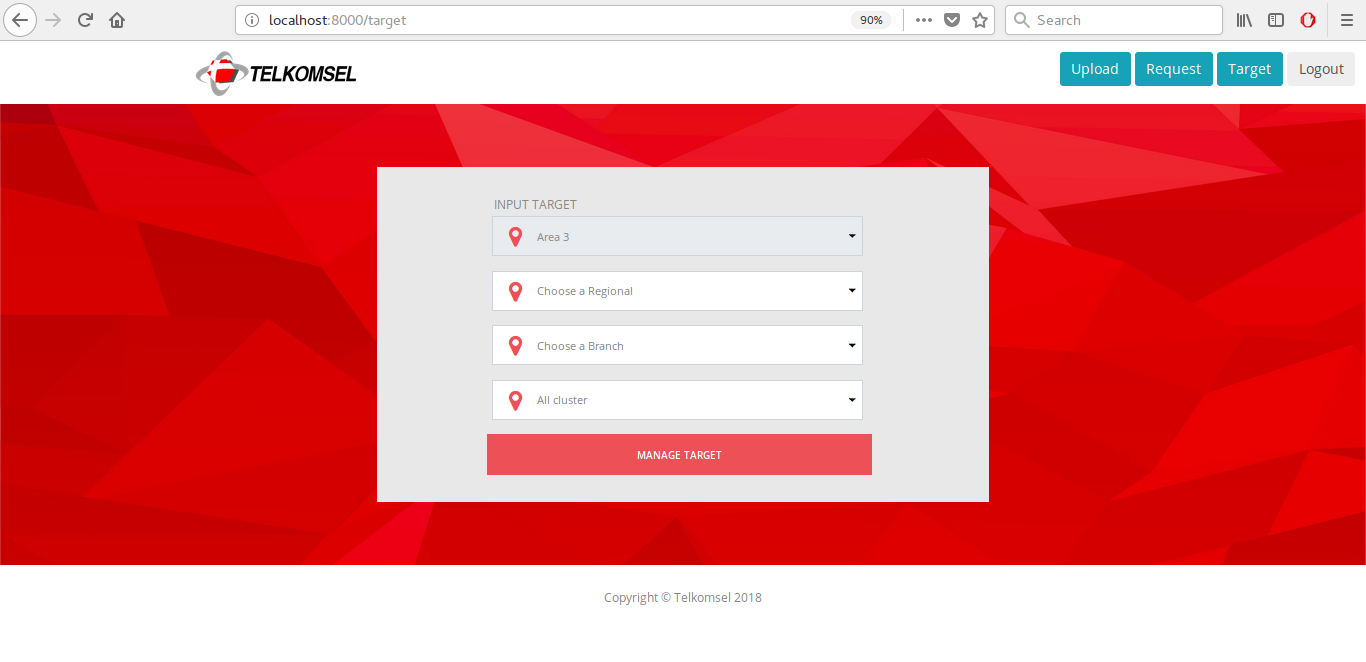
\includegraphics[width=10cm,height=5cm]{bab5/tampilanTarget.png}}
	\caption{Potongan Halaman Target TPORT}
	\label{figure:targetTPORT}
\end{figure}

\begin{figure}[h!]
	\centerline
	{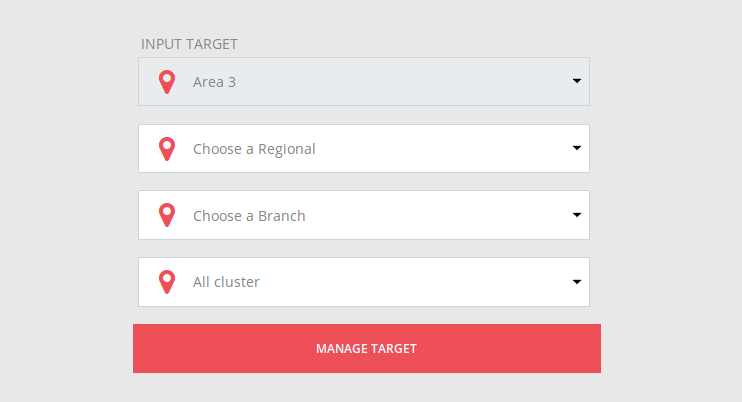
\includegraphics[width=10.5cm,height=6cm]{bab5/detailTampilanTarget.png}}
	\caption{Potongan Halaman Target TPORT}
	\label{figure:detailTargetTPORT}
\end{figure}

\subsection{Halaman Pencapaian \textit{Revenue}}
Pada halaman pencapaian \textit{revenue} bahasa pemrograman yang digunakan adalah HTML, CSS dan PHP. Pada halaman ini, pengguna dapat melihat detail pencapaian \textit{revenue} berdasarkan wilayah, tanggal, dan kategori yang dipilih. Halaman ini akan menampilkan detail informasi sesuai pilihan pengguna tadi. Gambar \ref{figure:pencapaianTPORT} dan \ref{figure:detailPencapaianTPORT} adalah tampilan halaman dan \ref{lst:pencapaianTPORT} adalah potongan kode dari halaman detail pencapaian \textit{revenue}.

\begin{figure}[h!]
	\centerline
	{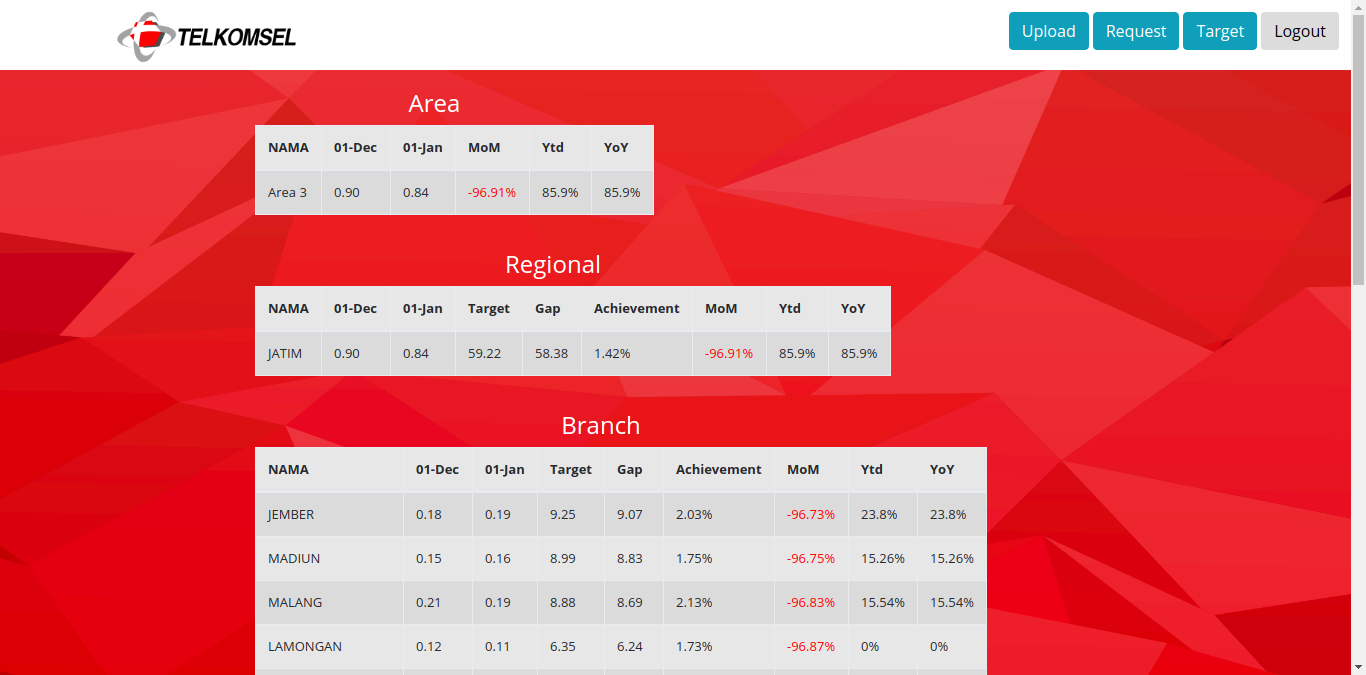
\includegraphics[width=10cm,height=5cm]{bab5/tampilanDetailPencapaian.png}}
	\caption{Halaman Detail Pencapaian \textit{Revenue}}
	\label{figure:pencapaianTPORT}
\end{figure}

\begin{figure}[h!]
	\centerline
	{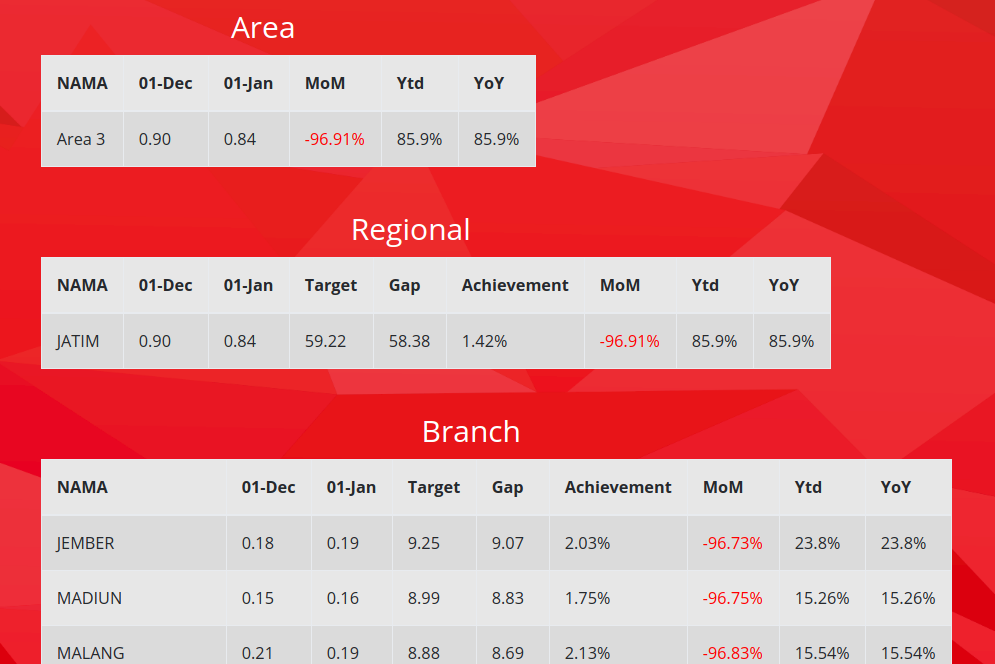
\includegraphics[width=9cm,height=6cm]{bab5/detailTampilanPencapaian.png}}
	\caption{Detail Halaman Pencapaian \textit{Revenue}}
	\label{figure:detailPencapaianTPORT}
\end{figure}

\lstinputlisting[language=PHP, firstline=1, lastline=24, firstnumber=1, caption=Potongan Kode Tampilan Target TPORT, label={lst:pencapaianTPORT}]{bab5/src/halamanDetail.php}

	\chapter{HASIL DAN UJI COBA}
Pada bab ini akan dipaparkan hasil uji coba saat sistem dijalankan. Uji coba sistem TPORT akan dilakukan untuk memastikan kualitas perangkat lunak yang dikembangkan dengan analisis dan perancangan perangkat lunak.
\section{Lingkungan Uji Coba}
Lingkungan uji coba sistem pada Kerja Praktik kali ini meliputi perangkat keras dan perangkat lunak adalah sebagai berikut:
\begin{enumerate}
	\item Perangkat Keras
	\begin{itemize}
		\item \textit{Processor} Intel® Core™ i7-5500U CPU @ 2.40GHz
		\item Memori 4 GB
	\end{itemize}
	\item Perangkat Lunak
	\begin{itemize}
		\item Sistem Operasi Ubuntu 16.04 LTS 64 bit.
	\end{itemize}
\end{enumerate}

\section{Skenario Pengujian}
Skenario pengujian yang akan dilakukan pada aplikasi TPORT adalah melakukan peran sebagai admin yang sedang membuka aplikasi. Langkah-langkah dari skenario adalah sebagai berikut:
	\begin{enumerate}
	\item Pengguna membuka aplikasi TPORT
	\item Pengguna memilih menu \textit{upload}, \textit{request}, dan target
	\item Pengguna menambahkan data pencapaian \textit{revenue} dengan mengupload file pada halaman upload
	\item Pengguna melihat detail hasil pencapaian \textit{revenue} pada halaman \textit{request}
	\end{enumerate}
	
\subsection{Pengujian Mengupload Data Pencapaian \textit{Revenue}}
Pengujian ini dilakukan terhadap fungsionalitas \textit{upload} data pencapaian \textit{revenue}. Tabel \ref{tab:list_upload} menjelaskan pengujian fungsionalitas ini.

\begin{table}[h!]
	\centering
	\begin{tabular}{|p{4cm}|p{6cm}|}
	\hline
	Kode \textit{Use Case} & UC-001\\ \hline
	Tujuan Pengujian & \textit{Upload} semua data hasil pencapaian \textit{revenue}\\ \hline
	Data Masukan & File .csv \\ \hline
	Prosedur Pengujian & 
		\begin{enumerate}
		\item Pengguna \textit{login} sebagai administrator
		\item Pengguna memilih menu \textit{upload}
		\end{enumerate}\\ \hline
	Hasil yang diharapkan & Semua data hasil pencapaian \textit{revenue} dapat di-\textit{upload} dan data yang di-\textit{upload} dapat masuk ke basis data sistem \\ \hline
	Hasil yang diperoleh & Semua data hasil pencapaian \textit{revenue} dapat di-\textit{upload} dan masuk ke basis data sistem \\ \hline
	Kesimpulan & Proses \textit{upload} hasil pencapaian \textit{revenue} berhasil \\ \hline
	Kondisi Akhir & Data hasil pencapaian \textit{revenue} masuk ke basis data sistem\\ \hline
	\end{tabular}\caption{Skenario Pengujian \textit{Upload} Data Hasil Pencapaian \textit{Revenue}}
	\label{tab:list_upload}
\end{table}

\subsection{Pengujian Mengelola Target Pencapaian \textit{Revenue}}
Pengujian ini dilakukan terhadap fungsionalitas mengelola target pencapaian \textit{revenue}. Tabel \ref{tab:list_target} menjelaskan pengujian fungsionalitas ini. Gambar \ref{figure:lihatTarget} adalah hasil fungsionalitas menampilkan target serta mengubah target.

\begin{figure}[h!]
\centerline
{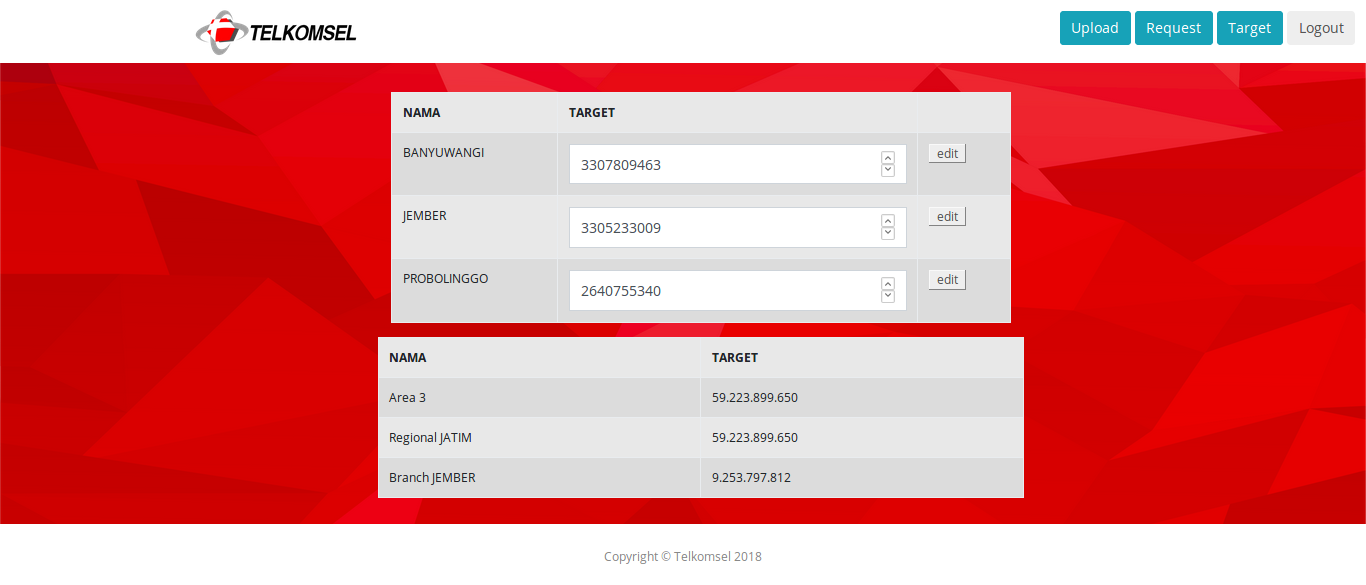
\includegraphics[width=10cm,height=5cm]{bab6/halamanTarget.png}}
\caption{Detail Data Target}
\label{figure:lihatTarget}
\end{figure}

\begin{table}[h!]
	\centering
	\begin{tabular}{|p{4cm}|p{6cm}|}
	\hline
	Kode \textit{Use Case} & UC-002\\ \hline
	Tujuan Pengujian & Menampilkan dan mengubah target pencapaian \textit{revenue}\\ \hline
	Data Masukan & - \\ \hline
	Prosedur Pengujian & 
		\begin{enumerate}
		\item Pengguna \textit{login} sebagai administrator
		\item Pengguna memilih menu target
		\end{enumerate}\\ \hline
	Hasil yang diharapkan & Semua data target pencapaian \textit{revenue} dapat ditampilkan serta dapat diubah pada menu target \\ \hline
	Hasil yang diperoleh & Semua data target pencapaian \textit{revenue} dapat ditampilkan dan diubah \\ \hline
	Kesimpulan & Proses menampilkan dan mengubah data target pencapaian \textit{revenue} berhasil\\ \hline
	Kondisi Akhir & Pengguna mendapatkan semua informasi data target pencapaian serta dapat mengubahnya \textit{revenue}\\ \hline
	\end{tabular}\caption{Skenario Pengujian Menampilkan dan Mengubah Data Target Pencapaian \textit{Revenue}}
	\label{tab:list_target}
\end{table}

\subsection{Pengujian Menampilkan Hasil Pencapaian \textit{Revenue}}
Pengujian ini dilakukan terhadap fungsionalitas menampilkan hasil pencapaian \textit{revenue}. Tabel \ref{tab:list_request} menjelaskan pengujian fungsionalitas ini. Gambar \ref{figure:requestL1}, \ref{figure:requestL3}, dan \ref{figure:requestTop5} adalah hasil fungsionalitas menampilkan hasil pencapaian \textit{revenue}.

\begin{figure}[h!]
	\centerline
	{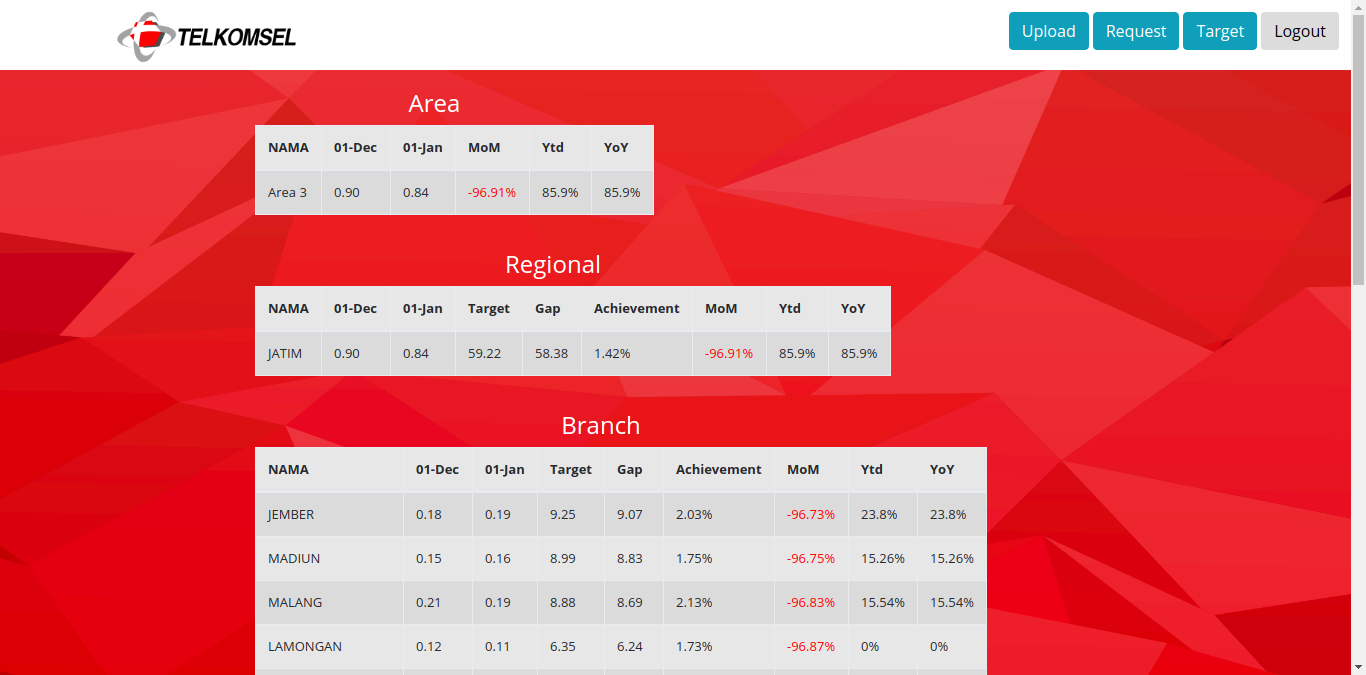
\includegraphics[width=10cm,height=5cm]{bab6/halamanL1.png}}
	\caption{Hasil Pencapaian \textit{Revenue} Berdasarkan L1}
	\label{figure:requestL1}
\end{figure}

\begin{figure}[h!]
	\centerline
	{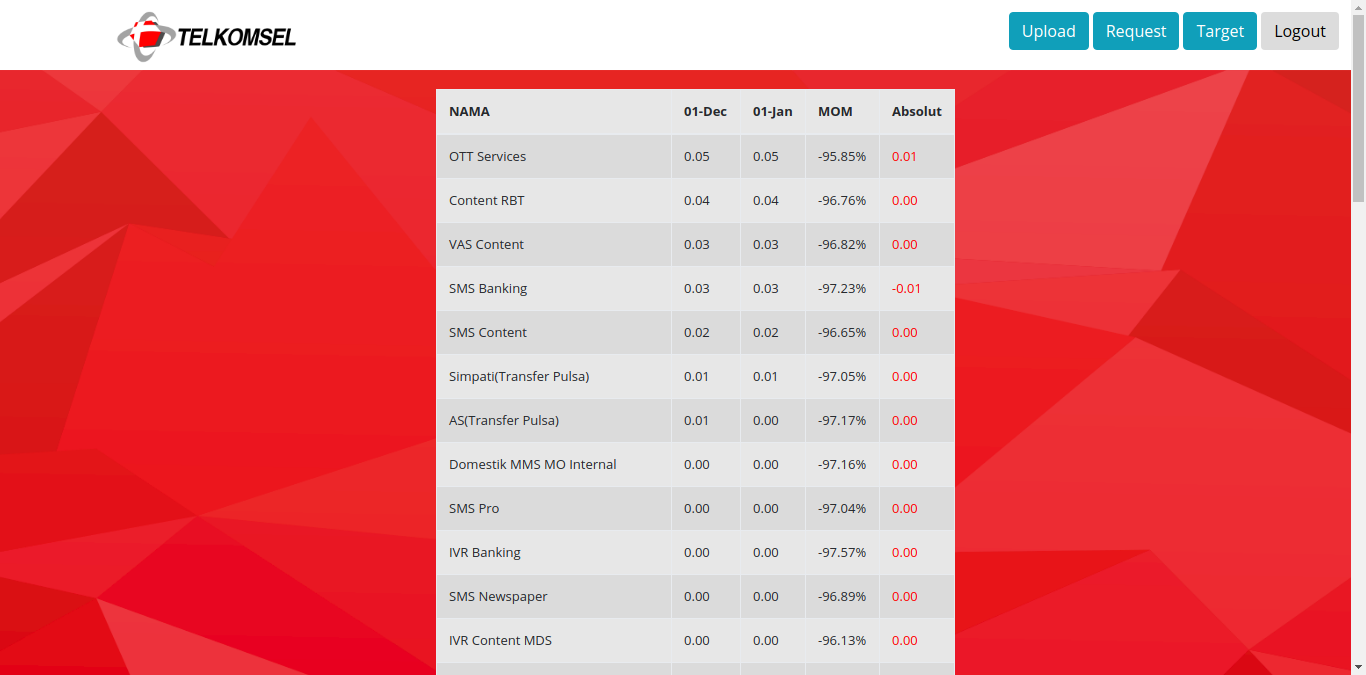
\includegraphics[width=10cm,height=5cm]{bab6/halamanL3.png}}
	\caption{Hasil Pencapaian \textit{Revenue} Berdasarkan L3}
	\label{figure:requestL3}
\end{figure}

\begin{figure}[h!]
	\centerline
	{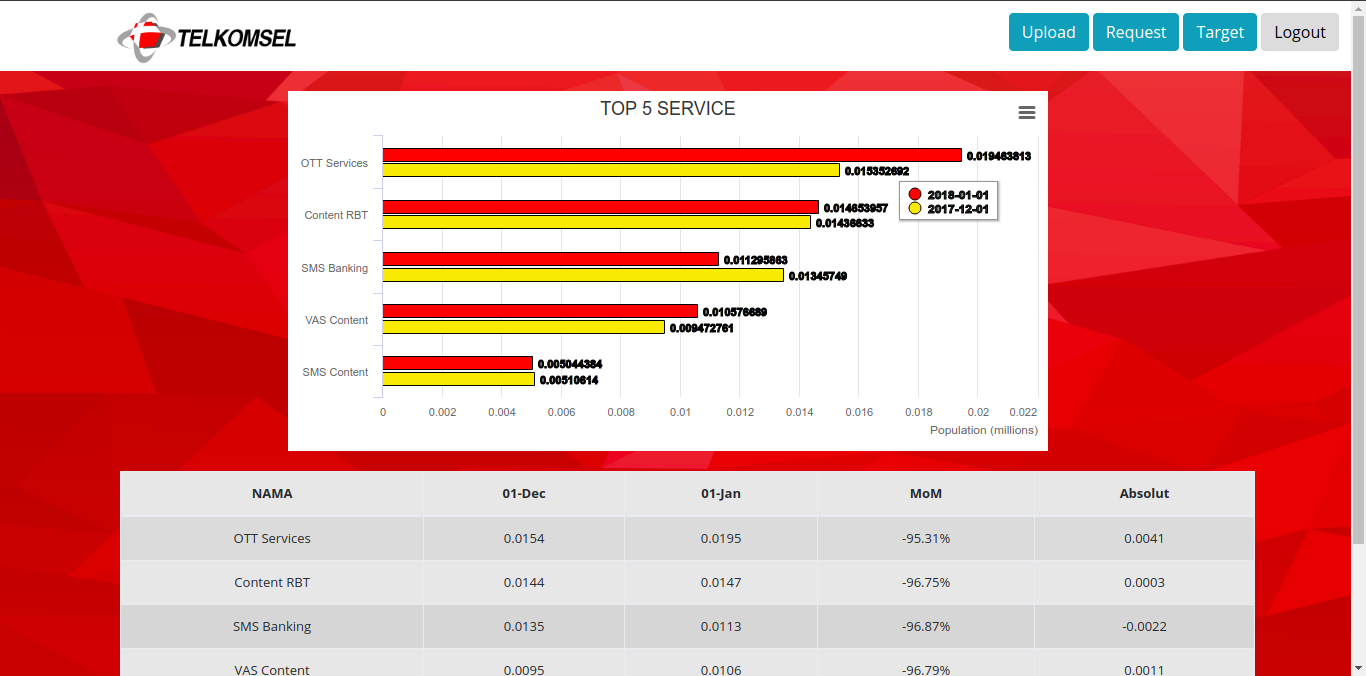
\includegraphics[width=10cm,height=5cm]{bab6/halamanT5.png}}
	\caption{Hasil Pencapaian \textit{Revenue} Berdasarkan Top 5}
	\label{figure:requestTop5}
\end{figure}

\begin{table}[h!]
	\centering
	\begin{tabular}{|p{4cm}|p{6cm}|}
		\hline
		Kode \textit{Use Case} & UC-003\\ \hline
		Tujuan Pengujian & Menampilkan hasil pencapaian \textit{revenue} berdasarkan L1, L3, dan Top 5\\ \hline
		Data Masukan & - \\ \hline
		Prosedur Pengujian & 
		\begin{enumerate}
			\item Pengguna \textit{login} sebagai administrator
			\item Pengguna memilih menu \textit{request}
		\end{enumerate}\\ \hline
		Hasil yang diharapkan & Semua hasil pencapaian \textit{revenue} berdasarkan L1, L3, dan Top5 dapat ditampilkan \\ \hline
		Hasil yang diperoleh & Semua hasil pencapaian \textit{revenue} berdasarkan L1, L3, dan Top5 dapat ditampilkan \\ \hline
		Kesimpulan & Proses menampilkan hasil pencapaian \textit{revenue} berdasarkan L1, L3, dan Top 5 berhasil\\ \hline
		Kondisi Akhir & Pengguna dapat melihat hasil pencapaian \textit{revenue} berdasarkan L1, L3, dan Top 5\\ \hline
	\end{tabular}\caption{Skenario Pengujian Menampilkan Hasil Pencapaian \textit{Revenue}}
	\label{tab:list_request}
\end{table}


\section{Evaluasi Pengujian}
\tab Hasil pengujian dihasilkan pengamatan lebih lanjut terhadap perilaku sistem \textit{Monitoring} SIK terhadap skenario kasus uji coba. Pengujian dilakukan \textit{internal team} untuk mencoba sistem yang telah diterapkan. Tabel \ref{tab:hasil_pengujian} adalah hasil pengujian pada sistem informasi \textit{monitoring} SIK.
\begin{table}[h!]
	\centering
	\begin{tabular}{|p{6cm}|p{4cm}|}
	\hline
	\textbf{Tugas} & \textbf{Hasil}\\ \hline
	Sistem mampu menampilkan informasi fitur-fitur \textit{Monitoring} SIK & Terpenuhi\\ \hline
	Sistem mampu menampilkan detail informasi kepada user & Terpenuhi\\ \hline
	Sistem mampu menangani pengelolaan data \textit{Monitoring} SIK & Terpenuhi\\ \hline
	Sistem mampu mengeksport data SIK ke dalam bentuk file berekstensi pdf & Terpenuhi\\ \hline
	Sistem menampilkan data sesuai dengan \textit{keyword} pencarian & Terpenuhi\\ \hline
	Sistem dapat mendownload dan upload file ke dalam basis data & Terpenuhi\\ \hline
	\end{tabular}\caption{Hasil Pengujian}
		\label{tab:hasil_pengujian}
\end{table}

Dengan hasil pengujian yang telah dilakukan, dapat disimpulkan bahwa keseluruhan aplikasi \textit{Monitoring} SIK memenuhi kriteria yang disebutkan pada sub-bab sebelumnya.

\section{Evaluasi Performa}
Tabel \ref{tab:evaluasi_performa_1} dan \ref{tab:evaluasi_performa_2} adalah hasil dari uji coba evaluasi performa sistem informasi \textit{monitoring} SIK.
\begin{table}
\centering
\begin{tabular}{|p{5cm}|p{2.5cm}|p{2cm}|}
\hline
\textbf{Tugas} & \textbf{Hasil} & \textbf{Waktu}\\ \hline
Membuka Halaman Dashboard & Terpenuhi & 2 detik\\ \hline
Membuka Halaman Request Relokasi & Terpenuhi & 1 detik\\ \hline
Menambahkan Request Relokasi & Terpenuhi & 2 detik\\ \hline
\end{tabular}\caption{Hasil Uji Performa(1)}
		\label{tab:evaluasi_performa_1}
\end{table}

\begin{table}
\centering
\begin{tabular}{|p{5cm}|p{2.5cm}|p{2cm}|}
\hline
\textbf{Tugas} & \textbf{Hasil} & \textbf{Waktu}\\ \hline
Membuka Halaman SIK & Terpenuhi & 1 detik\\ \hline
Menambahkan SIK & Terpenuhi & 2 detik\\ \hline
Membuka Halaman Penagihan & Terpenuhi & 1 detik\\ \hline
Menambahkan Penagihan & Terpenuhi & 2 detik\\ \hline
Membuka Halaman Eksekusi & Terpenuhi & 1 detik\\ \hline
Menambahkan Eksekusi & Terpenuhi & 2 detik\\ \hline
Membuka Halaman Finish & Terpenuhi & 1 detik\\ \hline
Menambahkan Finish & Terpenuhi & 2 detik\\ \hline
Mendownload Request Relokasi & Terpenuhi & 2 detik\\ \hline
Mendownload SIK & Terpenuhi & 2 detik\\ \hline
Mendownload Berita Acara & Terpenuhi & 2 detik\\ \hline
Mendownload Penagihan & Terpenuhi & 2 detik\\ \hline
\end{tabular}\caption{Hasil Uji Performa(2)}
		\label{tab:evaluasi_performa_2}
\end{table}

\vspace{4 cm}
\textcolor{white}{..}
	\chapter{KESIMPULAN DAN SARAN}

\section{Kesimpulan}
Kesimpulan dari Kerja Praktik kali ini adalah sebagai berikut:
\begin{enumerate}
\item Aplikasi \textit{Monitoring} SIK berhasil dibuat dengan menggunakan bahasa pemrograman HTML, CSS, Javascript dan PHP untuk dapat memenuhi kebutuhan standar dalam pengelolaan permintaan relokasi ATM BRI.
\item Penggunaan \textit{framework} Laravel dan BDMS MySQL berhasil diterapkan untuk membuat aplikasi \textit{Monitoring} SIK, yang sangat diperlukan untuk memantau kegiatan pengelolaan permintaan relokasi hingga pembayaran kegiatan relokasi ATM BRI.
\item Performa dari sistem informasi \textit{Monitoring} SIK memiliki performa yang baik dalam penanganan tugas yang dikerjakan menggunakan sistem yang telah dibuat.
\end{enumerate}

\section{Saran}
Setelah melalui Kerja Praktik kali ini, penulis memberikan saran sebagai berikut:
\begin{enumerate}
\item Tampilan \textit{front end} harus teroptimasi dengan baik pada seluruh \textit{device} dan \textit{browser}. Mengingat beragamnya \textit{device} dan \textit{browser} yang digunakan pengguna.
\item Perlu dilakukan penelitian terhadap segala pengembangan fitur sistem di masa mendatang.
\end{enumerate}
	
	\appendix
	\begin{thebibliography}{9}
	
	\bibitem{PHP}
	\textbf{PHP, "What is PHP?"} [Online]. Available: http://php.net/manual/en/intro-whatis.php. [Accessed 4 October 2017].		
	
	\bibitem{javascript}
	\textbf{What is JavaScript?}, Mozilla Developer Network. [Online]. Tersedia pada: https://developer.mozilla.org/en-US/docs/Learn/JavaScript/First\_steps/
	What\_is\_JavaScript. [Accessed 6 October 2017].
	
	\bibitem{laravel}
	\textbf{What is Laravel?}, Laravel (Project Using Symphony) [Online]. Available: https://symfony.com/projects/laravel. [Accessed 8 October 2017].
	
	\bibitem{sejarahtsel}
	\textbf{Sejarah Telkomsel}, Sejarah Telkomsel [Online]. Available: https://id.wikipedia.org/wiki/Telkomsel. [Accessed 17 March 2018].
	
	\bibitem{telkomsel}
	\textbf {Sejarah Telkomsel}, Sejarah Kami [Online]. Available: https://www.telkomsel.com/about-us/our-story/our-history. [Accessed 17 March 2018].
	
	\bibitem{aboutus}
	\textbf{Tentang Telkomsel}, Tentang Telkomsel [Online]. Available: https://www.telkomsel.com/about-us/our-story. [Accesed 17 March 2018].
	
	\bibitem{apache}
	\textbf {Apache HTTP Server}, What is the Apache HTTP Server Project?, [Online]. Available: https://en.wikipedia.org/wiki/Apache\_HTTP\_Server. [Accessed 19 December 2017].
	
	\bibitem{mysql}
	\textbf{MySQL}, [Online]. Available: http://www.oracle.com/technetwork/database/mysql/index.html. [Accessed 19 December 2017].
\end{thebibliography}

	\backmatter
	\chapter{BIODATA PENULIS}
\begin{wrapfigure}{l}{0.4\textwidth}
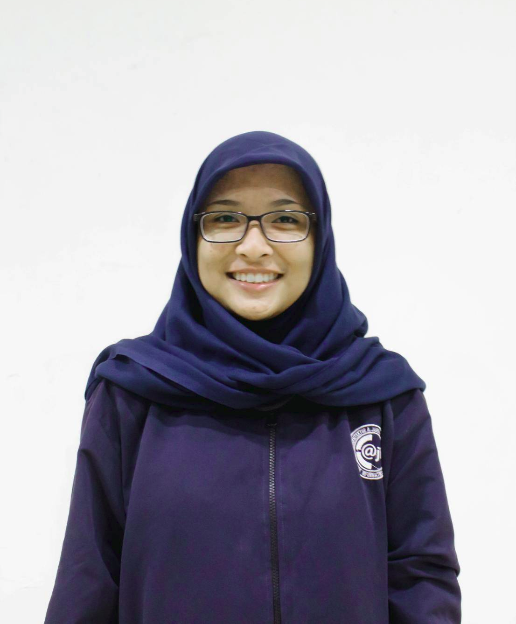
\includegraphics[height=0.3\textheight]{biodata/hana.png}
\end{wrapfigure}

\textbf{Rohana Qudus}, lahir di Gresik tanggal 7 Februari 1998. Penulis merupakan anak kedua dari 2 bersaudara. Penulis telah menempuh pendidikan formal TK Dharmawanita Gresik, SD Muhammadiyah 2 Gresik (2004-2010), SMP Negeri 1 Gresik (2010-2013) dan SMA Negeri 1 Gresik (2013-2015). Penulis melanjutkan studi kuliah program sarjana di Departemen Informatika ITS. 

Selama berkuliah di Departemen Informatika ITS, penulis  pernah menjadi asisten dosen dan praktikum untuk mata kuliah Sistem Operasi (2017) dan Jaringan Komputer(2018). Selama menempuh perkuliahan penulis juga aktif di kegiatan organisasi dan kepanitiaan diantaranya menjadi Staf Departemen Media Informasi HMTC ITS, Staf Departemen Informasi Informasi Media BEM FTIF ITS, Staf Ahli Departemen Media Informasi HMTC ITS, Staf Website dan Kesekretariatan Schematics 2016, dan Staf Ahli 3D Schematics 2017. Penulis dapat dihubungi melalui surel di \\ \texttt{rohanaq27@gmail.com}.

\chapter{BIODATA PENULIS} 
\begin{wrapfigure}{l}{0.4\textwidth} 
	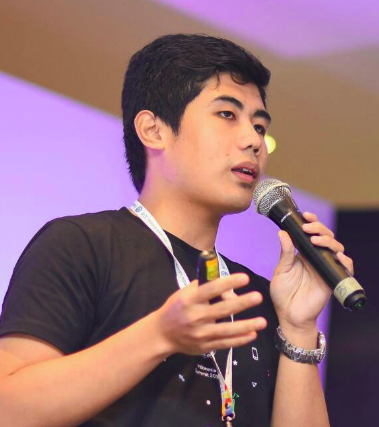
\includegraphics[height=0.3\textheight]{biodata/rafi.png} 
\end{wrapfigure} 

\textbf{Rafi R. Ramadhan}, lahir di Padang Panjang tanggal 27 Januari 1997. Penulis merupakan anak kedua dari 2 bersaudara. Penulis telah menempuh pendidikan formal TK Aisyiyah I Duri, Riau, SD IT Mutiara Duri (2003-2009), SMP IT Mutiara (2009-2012) dan SMA IT Mutiara Duri Riau (2012-2015). Penulis melanjutkan studi kuliah program sarjana di Jurusan Teknik Informatika ITS. 

Selama berkuliah di Departemen Informatika ITS, penulis aktif dalam kegiatan kemahasiswaan seperti Himpunan. Penulis merupakan staf pada Departemen Media dan Informasi HMTC 2016-2017, kemudian melanjutkan menjadi staf ahli pada departemen yang sama untuk periode 2017-2018. Selain di himpunan, penulis juga aktif pada Schematics selama 2 tahun berturut-turut. Penulis juga merupakan Volunteer dari International Office ITS. Penulis berada pada divisi Internationalization and Development Division, divisi ini mengemban tugas untuk mencerdaskan dan membantu proses internasionalisasi yang ada di kampus ITS. Penulis juga merupakan Leader dari Developer Student Clubs yang merupakan program gagasan dari Google Developer. penulis merupakan 1 dari 20 orang yang dipilih menjadi Leader untuk DSC se-Indonesia. Penulis dapat dihubungi melalui surel di \\ \texttt{rafi.ramadhan27@gmail.com}.
\end{document}
